%Question 1
\def \Rs{50 		\times 10^3}
\def \RL{400}
\def \Rione{1		\times 10^6}
\def \Roone{1		\times 10^3}
\def \Ritwo{200		\times 10^3}
\def \Rotwo{2		\times 10^3}
\def \Rithree{25	\times 10^3}
\def \Rothree{50}
\def \Aone{10}
\def \Atwo{100}
\def \Athree{2}

%Final A Matrix
\def \Aoneone{542.7		\times 10^{-6}}
\def \Aonetwo{27.135	\times 10^{-3}}
\def \Atwoone{542.7		\times 10^{-12}}
\def \Atwotwo{27.135 	\times 10^{-9}}

\def \Gtot{1559.9}

\begin{enumerate}
	
	%Part a
	\item{
	\text{}
	
	\begin{figure}[H]
	\begin{center}
	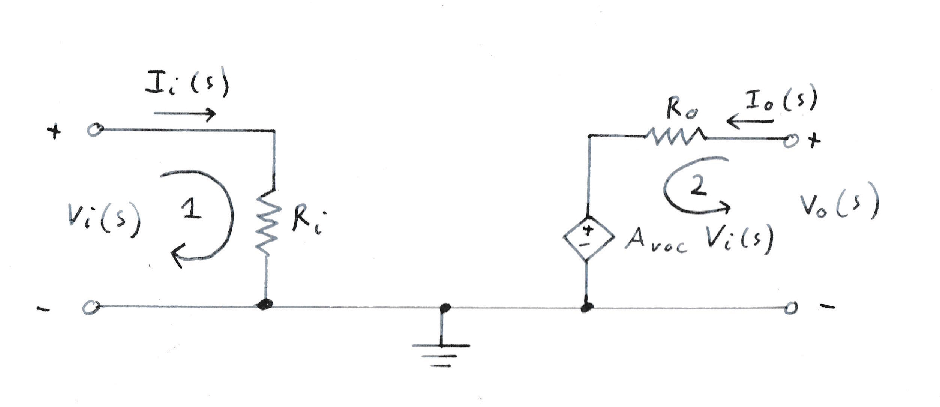
\includegraphics[scale=0.6]{q1_1.pdf}
	\end{center}
	\end{figure}
	
	Using KVL in loop 1:
	\begin{align*}
	&\Sigma V_{drops} = 0
	\\
	\implies & V_i + I_i R_i =0
	\\
	\implies & V_i = I_i R_i
	\end{align*}		
	
	Using KVL in loop 2:
	\begin{align*}
	&\Sigma V_{drops} = 0
	\\
	\implies & -V_o + I_o R_o + A_{voc}V_i = 0
	\\
	\implies & -V_o + I_o R_o + A_{voc}I_i R_i = 0
	\\
	\implies & I_i = \frac{V_o - I_o R_o}{A_{voc}R_i}
	\\
	\implies & V_i = \frac{V_o - I_o R_o}{A_{voc}}
	\end{align*}		
	
	We know that for a two port network, the general matrix
	equation written in $a$ parameters is:
	$$ \left[ \begin{matrix}
	V_i \\ 
	I_i
	\end{matrix}\right] = \left[ \begin{matrix}
	a_{11} & -a_{12} \\ 
	a_{21} & -a_{22}
	\end{matrix}  \right] \left[ \begin{matrix}
	V_o \\ 
	I_o
	\end{matrix}  \right]  $$	
	From the equation obtained before, we can re-write them in matrix form:
	$$ \left[ \begin{matrix}
	V_i \\ 
	I_i
	\end{matrix}\right] = \left[ \begin{matrix}
	\frac{1}{A_{voc}} 		& -\frac{R_o}{A_{voc}} \\[6pt] 
	\frac{1}{A_{voc}R_i}	& -\frac{R_o}{A_{voc}R_i}
	\end{matrix}  \right] \left[ \begin{matrix}
	V_o \\ 
	I_o
	\end{matrix}  \right]  $$	
	}
	Therefore, the $A$ matrix of this voltage amplifier model is:
	$$ A = 
	\left[ \begin{matrix}
	\frac{1}{A_{voc}} 		& \frac{R_o}{A_{voc}} \, \Omega \\[6pt] 
	\frac{1}{A_{voc}R_i} \, \mho	& \frac{R_o}{A_{voc}R_i}
	\end{matrix}  \right] $$
	\\
	
	%Part b
	\item{
	This circuit can be thought of as 3 cascaded two port networks forming 
	a single two port network with a loaded output and a voltage input with 
	source impedance.\\
	To find the $A$ parameter matrix of the single two port network, first 
	find the $A$ parameter matrices of each amplifier stage and matrix 
	multiply them together.
	
	\begin{align*}
	A_1 &= 
	\left[ \begin{matrix}
	\frac{1}{\Aone} 			& \frac{\Roone}{\Aone} \\[6pt] 
	\frac{1}{(\Aone) (\Rione) }	& \frac{\Roone}{(\Aone) (\Rione)}
	\end{matrix}  \right] 
	\\
	A_2 &= 
	\left[ \begin{matrix}
	\frac{1}{\Atwo} 			& \frac{\Rotwo}{\Atwo} \\[6pt] 
	\frac{1}{(\Atwo) (\Ritwo) }	& \frac{\Rotwo}{(\Atwo) (\Ritwo)}
	\end{matrix}  \right] 
	\\
	A_3 &= 
	\left[ \begin{matrix}
	\frac{1}{\Athree} 				& \frac{\Rothree}{\Athree} \\[6pt] 
	\frac{1}{(\Athree) (\Rithree) }	& \frac{\Rothree}{(\Athree) (\Rithree)}
	\end{matrix}  \right] 
	\\
	\\
	A &= A_1 A_2 A_3
	\\
	&= \left[ \begin{matrix}
	\Aoneone 			& \Aonetwo \; \Omega \\ 
	\Atwoone \; \mho \	& \Atwotwo
	\end{matrix}  \right]
	\end{align*}
	
	Now the circuit can be modelled like this:
	
	\begin{figure}[H]
	\begin{center}
	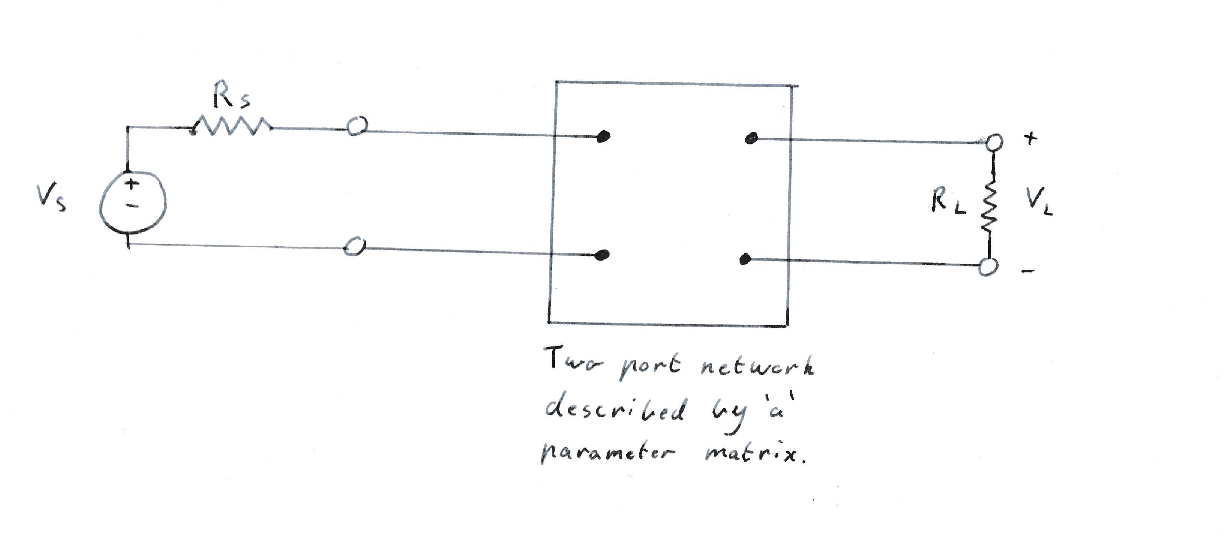
\includegraphics[scale=0.6]{q1_2.pdf}
	\end{center}
	\end{figure}
	
	Using Table 18.2 from the formula sheet, the formula
	
	$$ \frac{V_2}{V_g} = \frac{Z_L}{(a_{11} + a_{21}Z_g)Z_L + a_{12} + a_{22}Z_g} $$
	can be used here.
	
	\begin{align*}
	G &= \frac{v_L}{v_s}
	\\
	&= \frac{R_L}{(a_{11} + a_{21}R_s)R_L + a_{12} + a_{22}R_s}
	\\
	&= \frac{\RL}{(\Aoneone + (\Atwoone)(\Rs))(\RL) + \Aonetwo + (\Atwotwo)(\Rs)}
	\\ \\
	&= \Gtot \, \text{V/V}
	\\
	\end{align*}
	
	}
\end{enumerate}